\chapter{Monte-Carlo Methods}
\href{https://github.com/scaevolabars/monte-carlo}{Code Base}

\begin{heur}
	There is one useful thing that i found while making Monte-Carlo simulations.
	 Sometimes it is computatationaly costly to generate random variable from normal distribution and very good approximation for it
	 appeared to be Irwin-Hall distribution.
	 \begin{equation}
	 	X_n = \sum_{i = 0 }^{n} U_k  \quad \text{where} \quad U_k \quad \text{are independent random variables drawn from  uniform distribution} \quad U(0,1)
	 \end{equation}
 
 	The density function is given by:
 	\begin{equation}
 		f_{X}(x ; n)=\frac{1}{2(n-1) !} \sum_{k=0}^{n}(-1)^{k}\left(\begin{array}{l}
 			n \\
 			k
 		\end{array}\right)(x-k)^{n-1} \operatorname{sgn}(x-k)
 	\end{equation}
 	This pdf is basically piecewise polynomial function with $ \mu = \frac{n}{2}$ and $\sigma = \frac{n}{12}$.
 	
 	For $n = 12$ it gives good approximation for normal distribution pdf.
 	\begin{equation}
 		\phi(x) \approx \sqrt{\frac{12}{n}}(f_X(x;n) - \frac{n}{2}) - 6
 	\end{equation}
 
 	\begin{equation}
 		\phi(x) \approx f_X(x ; n) - 6 = \sum_{i = 0 }^{12} U_k
 	\end{equation}
 
 	% TODO:  required
 	\begin{figure}
 		\centering
 		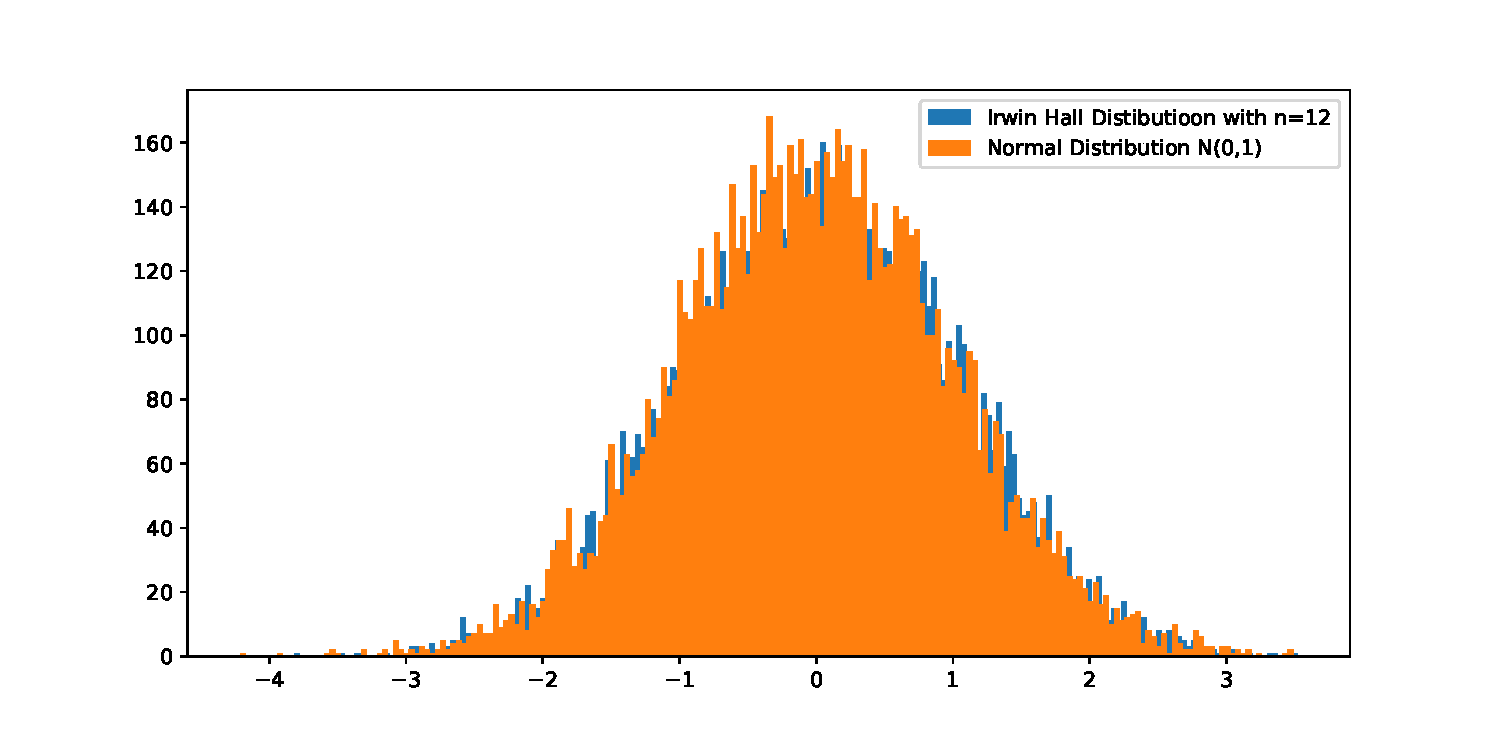
\includegraphics[width=0.8\linewidth]{numerical/figures/irwinhall}
 		\caption{}
 		\label{fig:irwinhall}
 	\end{figure}
 
 \section{Financial Instrument Pricing}
 \subsection{Black-Scholes Model}
 \begin{figure}
 	\centering
 	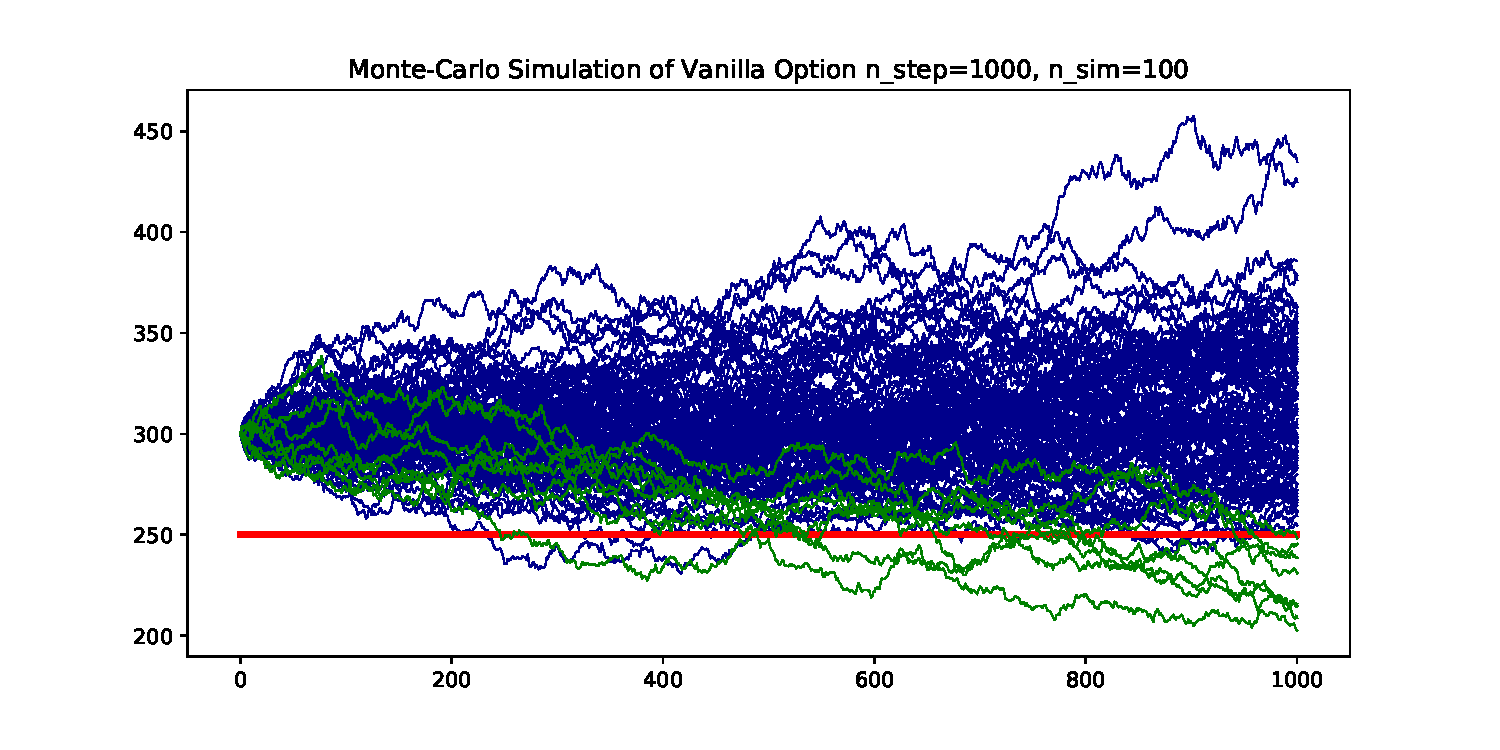
\includegraphics[width=0.8\linewidth]{numerical/figures/mcoption}
 	\caption{}
 	\label{fig:mcoption}
 \end{figure}
 
\end{heur}

\section{Metropolis-Hasting algorithm}
	Metropolis-Hasting (MH) algorithm arises in many contextes such as optimization, sampling from probability measure with unknown normalization. One of the benefits of this algorithm as it was said that it doesn't require measure to be normalized. The algorithm goes
	as follows:
	
	\subsection{Discrete}
	
	We are given a matrix $M_{ij}$ with positive entries s.t:
	\begin{equation}
		\forall i : 1 < i \le d  \sum_{ 1 < j \le d} M_{ij} = 1
	\end{equation}
	In other words every row sums up to $1$.
	
	Such matrices are called stochastic matrices or Markov chain transitions.
	
	Then we chooce initial random state $X_0$ and we define random variables $X_{n}$ taking values in $E = \left\{1, \ldots, d\right\}$
	by setting 
	\begin{equation}
		X_n = F_n(X_{n_1})	
	\end{equation}
	
	This sequence is called Markov chain taking values $E = \left\{1, \ldots, d\right\}$ with transition probabilities
	\begin{equation}
		\mathbb{P}\left(X_n = i \vert X_0 = j\right) =  M^n(i,j)
	\end{equation}
	\subsubsection{Steps}
	\begin{enumerate}
		\item We are given some line vector $\pi$ such that $\wedge_{i\in E} \pi(i) > 0$ and  $\sum_{ 1 < j \le d} \pi(j) = 1$. \\
		\item Choose the transition probablilty matrix $M(i,j)$ s.t $M(i,j) > 0$ and $M(j,i) > 0$ \\
		
		\item Set
		\begin{equation}
			a(i,j) = 1 \wedge \frac{\pi(i)M(i,j)}{\pi(j)M(j,i)} \in \left[0,1\right]
		\end{equation}
	
		\item On each step draw \textit{i.i.d.} $\left(U_n\right)_{n\ge 0}$ on $\left[0,1\right]$
		
		\item Run accesptence-rejection procedure
		 \begin{equation}
			X_{n-1} \rightsquigarrow Y_{n}=F_{n}\left(X_{n-1}\right) \rightsquigarrow X_{n}:=\left\{\begin{aligned}
				Y_{n} & \text { if } \quad U_{n} \leq a\left(X_{n-1}, Y_{n}\right) \\
				X_{n-1} & \text { if } \quad U_{n}>a\left(X_{n-1}, Y_{n}\right)
			\end{aligned}\right.
		\end{equation}
	\end{enumerate}
	
	The accepted sequence $X_n$ is the sample we needed.
	

	

	
	